\documentclass[12pt,letterpaper,english,bibliography=totocnumbered,abstract=on]{scrartcl}

\usepackage{indentfirst}
\usepackage{appendix}
\usepackage{fullpage}
%\usepackage{subfiles}
\usepackage[T1]{fontenc}
\usepackage[latin9]{inputenc}
\usepackage{color}
\usepackage{babel}
\usepackage{verbatim}
\usepackage[unicode=true,pdfusetitle,
bookmarks=true,bookmarksnumbered=false,bookmarksopen=false,
breaklinks=true,pdfborder={0 0 0},pdfborderstyle={},backref=false,colorlinks=true]
{hyperref}
\hypersetup{linkcolor=blue,citecolor=blue,urlcolor=blue}

\usepackage{booktabs}
\usepackage{multirow}
\usepackage{adjustbox}
\usepackage{threeparttable}
\usepackage[table]{xcolor}
\usepackage{csquotes}
\usepackage{soul} % for hiliting text: \hl
% old style is authoryear
\usepackage[backend=biber, style=numeric, maxbibnames=99]{biblatex}
\addbibresource{mylibrary.bib}
\addbibresource{CRB.bib}

\usepackage[disable]{todonotes}

% Prevent page breaks within paragraphs
% https://tex.stackexchange.com/questions/21983/how-to-avoid-page-breaks-inside-paragraphs
\widowpenalties 1 10000


\begin{document}
\titlehead{USDA-APHIS Progress Report}
\title{Coconut Rhinoceros Beetle Biological Control}
\author{Aubrey Moore, University of Guam}
\date{Submitted December 30, 2020\\Revised January 28, 2021}
\maketitle
\begin{description}	
	\item[Report ID:] AP19PPQS\&T00C168-PE-SA2-20 (RPT-46135)
	\item[Report Type:] Semiannual performance report
	\item[Performance Period:] August 8, 2019 - August 21, 2020
	\item[Federal Award Identification Number:] AP19PPQS\&T00C168
	\item[Agreement Title:] PPA7721 6R.0117.00 Guam CRB BC
\end{description}

\begin{footnotesize}
\url{https://github.com/aubreymoore/FY19-PPA-Report-1/raw/master/PPA19-report2.pdf}
\end{footnotesize}

\newpage{}
\tableofcontents{}

\newpage
\listoftodos

\newpage

\section{Abstract}
	\todo[color=green]{add new stuff}
	
	
	\textbf{CRB Biological Control.} The primary objective of this project was to find an isolate of \textit{Oryctes rhinoceros} nudivirus (OrNV) which can be used as an effective biological control agent for the CRB-G biotype of coconut rhinoceros beetle (CRB). 
	
	Laboratory bioassays indicated that OrNV from two sources could be considered as potential biocontrol agents for CRB-G: OrNV isolate V23B maintained in insect tissue culture by AgResearch New Zealand and OrNV in bodies of CRB collected in Taiwan for the current project. However, these laboratory studies did not indicate a level of efficacy deemed necessary to justify field release. Search for an effective biocontrol agent for CRB-G continues. 
	
	PCR tests of CRB-G adults collected on Guam during 2019 and early 2020 indicated presence of OrNV in this population. Results from a 2020 survey which followed an experimental protocol developed to minimize false positive test results for OrNV infection indicate that the Guam CRB is free from OrNV infection.  It is likely that positive PCR tests where the result of laboratory contamination. 	
	
	
	\textbf{CRB Damage Survey.} A secondary objective of this project was to develop a CRB damage monitoring system based on automated digital image analysis of roadside video surveys.
	
	Georeferenced videos were recorded using a smart phone mounted on a road vehicle. An object detector was trained to locate and provide a damage index (0 to 4) for all coconut palms in the videos. A second object detector was trained to locate v-shaped cuts, which are characteristic symptoms of CRB damage.
	
	The first island-wide roadside video survey of CRB damage on Guam was performed in early October 2020.  This survey yielded a damage index for each of 57,666 coconut palm images detected in 174,944 video frames. Nineteen percent of these palms were damaged. An online interactive map of the survey results is publicly available. The Guam survey will be repeated bimonthly to monitor spatial-temporal changes in CRB damage in response to control activities.
	
	A roadside video survey of Rota Island is currently being performed to test this survey method for early detection of CRB damage in areas where this pest is not known to be established.
	

	\textbf{Regional Collaboration.} CRB-G invasions are a major problem for Pacific islands. Uncontrolled outbreaks of this highly invasive biotype are damaging and killing palms in Guam, Rota, Hawaii, Palau, Papua New Guinea, and the Solomon Islands. Without effective control of these outbreaks, the problem will spread to other Pacific islands, resulting in a human tragedy when it reaches atolls were islanders still rely on coconut palm as the \textit{tree of life}. 
	
	Project resources, time and effort were used to facilitate communication among an \textit{ad hoc} collaboration of entomologists working on the CRB-G problem throughout the Pacific. Project staff have been active members of the CRB-G Action Group and have participated in annual scientific meetings organized by this group. The 2020 Action Group meeting was organized by Trevor Jackson at AgResearch New Zealand and Aubrey Moore at the University of Guam and run as a Zoom webinar. Recordings of all sections are available online. 
	
	This project has provided online resources including a searchable, online bibliography of journal articles and technical reports about CRB, an online interactive map for visualizing CRB invasion history, and a listserv to facilitate rapid informal exchange of technical and scientific information among people working on the CRB problem throughout the Pacific.


\section{Background}

The major goal of this project was to find an effective biological
control agent for coconut rhinoceros beetle biotype G (CRB-G).

Prior to arrival of CRB-G on Guam during 2007, coconut rhinoceros beetle
infestations of Pacific islands were readily dealt with by classical
biological control using \textit{Oryctes} nudivirus (OrNV), a pathogen specific to rhinoceros beetles. 
Following a lack
of response to release of OrNV on Guam, research showed that the Guam
CRB population is a genetically distinct virus-resistant biotype which
has become known as CRB-G \cite{marshall_new_2017-1}. This biotype is highly invasive and is
causing massive damage to coconut and oil palms after recent invasion of Papua New Guinea
and the Solomon Islands. CRB-G has also invaded Oahu and Rota. Eradication
attempts have been launched on these two islands.

Additional goals for this project were to establish a CRB damage survey to evaluate efficacy of biocontrol and other tactics, and to maintain and facilitate collaboration with other Pacific island entomologists working to find solutions for CRB-G management.

\section{Staffing}

Staff for this project comprised of the PI, a post-doc and a technician. 

\begin{itemize}
	
\item Funding from the Department of Interior, Office of Island Affairs
was used to hire an insect pathologist for a 2 year term. Dr. James
Grasela was recruited and started work at UOG on June 24, 2018.

\item Funding from this USDA-APHIS project was used to hire Mr. Chris Cayanan as a technician. Mr. Cayanan was hired during December, 2019, as a replacement for Mr. Ian Iriarte who resigned to accept another job.

\end{itemize}

\section{Biological Control}

\subsection{Laboratory Bioassays of OrNV Isolates}

Four isolates of OrNV were evaluated as candidate biological control agents for CRB-G in a series of laboratory bioassays. Virus sample preparations came from Dr. Sean Marshall's lab at AgResearch New Zealand were they are maintained in insect cell culture.

\begin{description}
	\item[DUG42] Collected from Dumaguete, Negros Island, Philippines in 2017
	\item[MALB] Collected from Malaysia, details not available.
	\item[PNG] Collected from Rabaul, Papua New Guinea in 1988
	\item[V23B] Collected from southern Luzon, Philippines in 1980
\end{description}

During laboratory bioassays, we dosed CRB-G adults with samples of the OrNV islolates, and observed mortality and changes in mass for one month. Each beetle was kept in isolation and individual records were stored in a laboratory information system developed for this application (Section \ref{lims}).



Bioassay results, displayed in Table \ref{tab: bioassay results}, indicate that one of the isolates, V23B, is pathogenic for CRB-G when doses are applied by placing droplets of virus suspension on mouthparts of adult beetles.


% Please add the following required packages to your document preamble:
% \usepackage{booktabs}
% \usepackage{multirow}
\begin{table}[h]
	\begin{adjustbox}{width=\columnwidth,center}
		
		\begin{threeparttable} 
			\caption{\textit{Oryctes rhinoceros} nudivirus (OrNV) bioassay results summary.}
			\label{tab: bioassay results}
			
			
			\begin{tabular}{ l l l c c c c }
				\toprule
				OrNV                  & bioassay                                        & method\tnote{1} & beetles & replicates & virus                           & inactivated                     \\
				isolate               &                                                 &                 &         &            & mortality (\textit{p})\tnote{2} & virus                           \\
				&                                                 &                 &         &            &                                 & mortality (\textit{p})\tnote{3} \\ \bottomrule
				DUG42                 & DUG42 \parencite{moore_bioassay_2019}                 & injection       & 30      & 2          & 40\% (0.65)                     & 40\% (0.65)                     \\ \midrule
				\multirow{2}{*}{MALB} & MALB \parencite{moore_bioassay_2019-6}                & injection       & 30      & 2          & 50\% (0.37)                     & \hphantom{0}0\% (1.00)          \\
				& MALBperOS \parencite{moore_bioassay_2019-7}           & per os          & 13      & 1          & -60\% (1.00)                    & 20\% (1.00)                     \\ \midrule
				\multirow{2}{*}{PNG}  & PNG \parencite{moore_bioassay_2019-2}                 & injection       & 81      & 4          & \cellcolor{yellow}{90\% (0.00)} & \hphantom{0}5\% (1.00)          \\
				& PNGperOS \parencite{moore_bioassay_2019-9}            & per os          & 21      & 1          & \hphantom{0}0\% (1.00)          & \hphantom{0} 0\% (1.00)         \\ \midrule
				\multirow{4}{*}{V23B} & V23B \parencite{moore_bioassay_2019-3}                & injection       & 66      & 4          & \cellcolor{yellow}{88\% (0.00)} & \hphantom{0}0\% (1.00)          \\
				& V23BperOS \parencite{moore_bioassay_2019-5}           & per os          & 32      & 2          & 80\% (0.07)                     & 20\% (0.69)                     \\
				& V23-large\_bioassay \parencite{moore_bioassay_2019-4} & per os          & 53      & 1          & \cellcolor{yellow}{42\% (0.00)} & -                               \\
				& V23\_perOSIN \parencite{moore_bioassay_2019-1}        & per os          & 16      & 1          & 60\% (0.06)                     & -                               \\ \bottomrule
			\end{tabular}
			\begin{tablenotes}[para]
				\item[1] Adult beetles were dosed either by direct injection of virus suspension into the haemocoel or by applying a droplet containing virus to mouthparts. \\ 
				\item[2] Percent mortality in beetles treated with virus, adjusted for untreated control mortality; 
				number in parentheses is the \textit{p}-value resulting from a Fisher's exact test of significant difference between mortality of treated and untreated beetles. \\
				\item[3] Percent mortality in beetles treated with heat inactivated virus, adjusted for untreated control mortality; 
				number in parentheses is the \textit{p}-value resulting from a Fisher's exact test of significant difference between mortality of treated and untreated beetles. 
			\end{tablenotes}
			
		\end{threeparttable}
	\end{adjustbox}
\end{table}

In a separate experiment, macerated guts from OrNV infected beetles from field collections of CRB in Taiwan were fed to CRB-G field-collected on Guam. PCR results indicated that the Taiwanese OrNV propagated in the Guam beetles (See Subsection \ref{(subsec: pcr results)}).

We now have two isolates of OrNV which can be considered as candidate biocontrol agents for further testing: V23B and Taiwan. 

\subsection{Virus Transmission Experiment}
\label{sec: virus transmission expt}

This experiment was performed to determine if OrNV isolate V23B can be transmitted from a dosed CRB adult to an undosed CRB adult. If a virus is not contagious in the lab, it will probably have no potential as a biocontrol agent. 

Unfortunately, the experiment failed due to very high mortality in the experimental control group and results are inconclusive. For details, see \cite{grasela_guam_2020}. This experiment needs to be repeated using pathogen-free, laboratory-reared adults (See Section \ref{sec: rearing}).

\subsection{PCR Tests for OrNV Detection}
\label{sec: pcr}

Previously, our laboratory relied on outside collaboration for molecular testing to determine presence of OrNV in CRB tissues. We recently acquired access to equipment and supplies which allow us to use PCR (polymerase chain reaction) techniques for OrNV detection. We tested five different primer pairs for detection of OrNV in reference samples from AgResearch New Zealand and were successful with all five. Identity of DNA fragments was confirmed as OrNV using a commercial DNA sequencing service.

Details of our PCR technique and initial series of tests can be found in \cite{grasela_technical_2020}, 
\cite{grasela_technical_2020-1} and \cite{grasela_technical_2020-2}.

Results from PCR tests indicate:
\label{(subsec: pcr results)}

\begin{itemize}

\item OrNV is present in the Guam adult CRB population: 18\% (10 of 47) gut samples dissected from field collected CRB tested positive for OrNV. \textbf{Important Note:} A recent field survey did not detect OrNV in the Guam CRB population. Most likely, positive PCR tests were a result of laboratory contamination. See the next section.

\item  OrNV is present in the adult Taiwanese CRB population:  7\% (5 of 67) gut samples dissected from field collected CRB tested positive for OrNV. 

\item  OrNV from Taiwanese adult CRB propagates in Guam adult CRB: 12\% (5 of 41) Guam CRB adults dosed with Taiwanese gut preparations tested positive.   

\end{itemize}

\subsection{Survey to Determine Incidence of OrNV Infection in the Guam CRB Population}

A survey to determine incidence of OrNV infection in the Guam CRB population was performed following positive PCR tests for OrNV infection in 18\% (10 of 47) gut samples dissected from locally collected beetles. The survey followed an experimental protocol developed to minimize false positive test results for OrNV infection is detailed in (\cite{mooreExperimentalPlanDetermining2020}).  Analysis of specimens collected during the survey is not yet complete because of our courier service temporarily lost one package of insects sent to AgResearch New Zealand. To date 104 of 200 CRB specimens collected in pheromone traps on Guam have been genotyped by CO1 DNA barcoding and tested for OrNV infection using PCR. All of these specimens were identified as CRB-G and none of them tested positive for OrNV. 

Preliminary survey results (\cite{graselaInvestigationDeterminePresence2020} and Marshall 2020, personal communication) indicate that previous PCR tests of field collected beetles on Guam which were positive for OrNV infection were most likely caused by laboratory contamination.

\subsection{CRB Rearing}
\label{sec: rearing}

\todo{Refer to new plans for a CRB rearing program.}

The CRB rearing program at UOG is being re-evaluated (see \cite{mooreIdeasReestablishmentCRB2020}).

Currently, experimental beetles were field-collected on Guam as prepupae, pupae or adults from breeding sites or as adults from pheromone traps.  Each beetle was given a serial number and was reared individually in a Mason jar stored in one of three environmental chambers set for 30 degrees Celsius, 80\% relative humidity and 12 hour photoperiod. Each adult beetle was fed weekly with a slice of banana. Detailed information on the CRB rearing facility can be found in a document prepared in support of a USDA-APHIS permit to allow importation of live CRB for laboratory bioassays \parencite{moore_additional_2019}.

\subsubsection{Urgent Need for a Pathogen-free CRB Laboratory Colony} 

To date, CRB used in bioassays and other laboratory experiments were field collected on Guam, rather than reared in a laboratory colony. This was done because a very high population density of rhino beetles on Guam made field collection far more efficient in terms of time and resources than laboratory rearing. However, field collected beetles are often infected with pathogens, especially the fungus, \textit{Anisopliae majus}, which was introduced on Guam as a classical biological control agent. Presence of these pathogens in experimental animals resulted in unpredictable and often high mortality rates in experimental control groups, leading to inconclusive results  such as experienced with the recent virus transmission experiment (\ref{sec: virus transmission expt}).

\subsubsection{Laboratory Information Management System}\label{lims}

We developed an online database which we use as a laboratory information management system for maintaining individual records for beetles in our rearing program \parencite{moore_coconut_2019-1}. This system was developed using the \href{http://www.web2py.com/}{web2py python web framework} and it is available on the web at \url{http://aubreymoore.pythonanywhere.com/rearing3}. 

\label{susceptible_biotype}
\subsubsection{Acquisition of a Virus-Susceptible CRB Biotype for Comparative Bioassays}

Since discovery of the CRB-G biotype on Guam \parencite{marshall_new_2017-1}, we have been operating under the hypothesis that this biotype is significantly more tolerant (resistant) to pathogenic effects of OrNV isolates previously used as effective biocontrol agents for CRB invading Pacific Islands. It has also been hypothesized that CRB-G has different behavioral characteristics, such as a significantly reduced attraction to oryctalure. However, comparative laboratory bioassays have not been performed to test these hypotheses.

We applied for and have been granted a USDA-APHIS import permit for live CRB which will allow us to establish a laboratory colony of CRB from presumed non-virus-resistant populations (See \parencite{moore_additional_2019} and \parencite{usda-aphis_crb_2019}). We have designed custom shipping containers to facilitate secure transport of live CRB \parencite{moore_container_2017-1}.

We plan to import CRB from American Samoa with assistance from our collaborator, Dr. Mark Schmaedick, American Samoa Community College. Plans for project staff to visit American Samoa in December 2019 failed because of travel restrictions prompted by a measles outbreak and in March 2020 because of travel restrictions prompted by the corona virus pandemic. 

\newpage
\subsection{Impediments to Progress in the Guam CRB Biocontrol Program}

Significant progress was made on the \textbf{Damage Survey} and \textbf{Regional Collaboration} components of this grant. However, progress on the \textbf{Biological Control} component is lagging because of travel restrictions, \textit{stay at home} orders, and a major technical problem. 

\subsubsection{Delays Caused by Travel Restrictions}

The original work plan included foreign travel to collect novel OrNV isolates for evaluation as biocontrol agents and to collect virus susceptible CRB biotypes for comparative bioassays. Our first planned collecting trip was to visit American Samoa in December 2019. This trip was canceled at the last minute because of a measles outbreak. Our second attempt, in March 2020 was also canceled at the last minute, because of COVID-19 travel restrictions. 

\subsubsection{Delays Caused by COVID-19 Stay-at-Home Orders and University Closures}

Progress was further delayed by Government of Guam \textit{stay at home} orders. The University of Guam was officially closed from March 20 to May 10 2020 and again from August 16 2020 to January 15 2021.

\subsubsection{Delays Caused by Detection of OrNV in CRB Collected on Guam}

%\subsection{PCR Tests for OrNV Detection}
%\label{sec: pcr}

Our lab currently uses CRB-G adults collected from pheromone traps as test animals in bioassays evaluating OrNV isolates as biocontrol agents under the assumption that the Guam beetle population contains only the CRB-G biotype and is free from OrNV infection. In 2019 we gained the capacity to perform PCR in our lab began testing these assumptions. PCR results indicated that field-collected beetles were all CRB-G, but 18\% of these tested positive for OrNV.

Based on these results, the PI decided to suspend bioassays until we had conclusive evidence of OrNV infection in the Guam CRB-G population.  An experimental plan \cite{mooreExperimentalPlanDetermining2020} was developed and executed. One hundred beetles were collected from each of two trapping sites (Leo Palace Resort in Southern Guam and the UOG Ag. Expt. Stn. in northern Guam). Gut samples were obtained from these beetles and tested using PCR in our lab and also in Sean Marshall's lab at AgResearch New Zealand. In PCR results from both labs all beetles tested positive for CRB-G biotype and negative for OrNV infection. We suspect that previous OrNV positive tests were the result of lab contamination (not false positives). 

During the hiatus in OrNV bioassays, we re-eximined our bioassay methodology and have decided to make major changes before moving forward:

\begin{itemize}
	\item \textbf{Re-establishment of a CRB rearing program.} High variance among bioassay replicates and high mortality rates are a serious impediment to progress in finding an OrNV isolate which can be used as an effective biocontrol agent for CRB-G. Beetles collected from pheromone traps are not ideal test insects because they vary in age and many are infected with \textit{Metarhizium majus}. 
	
	We intend to re-establish the Guam CRB rearing program to supply healthy, standardized test insects. Insects will be reared individually in Mason jars and a detailed record will be maintained for each individual. Larvae will be fed a diet of heat-sterilized CRB breeding site material from dead standing coconut trunks. The CRB-G lab colony will be initiated with surface-sterilized eggs and isofemale lineages will be maintained.
	
	Because the life cycle of the coconut rhinoceros beetle is about 9 months, there will be a lag time of about one year before the rearing program is fully operationaland bioassays can resume.	
	  
	\item \textbf{Measurement of sublethal impacts of OrNV infection.} The literature indicates that reduction in damage to coconut palms after release of OrNV may be the result of sublethal impacts on the population rather than mortality. These impacts may include reduction in fecundity, feeding, and flight. Bioassays which measure only mortality may reject promising biocontrol candidates.
	
	We already indirectly track feeding by weighing beetles during bioassays but will also include egg counts in future observations. We are considering using flight mills.
	  
	\item \textbf{Acquisition of virus susceptible biotypes.} One or more lab colonies of virus-susceptible biotypes are required for comparative bioassays (See section \ref{susceptible_biotype}). We originally planned to source non-CRB-G beetles during foreign exploration for OrNV isolates, but this has not happened because of COVID-19 travel restrictions. 
	
	Our new plan is to import gravid females from places such as Palau, where one or more virus-susceptible biotypes are known to exist, in addition to CRB-G. Eggs from these females will be used to establish isofemale lineages and these lines will be genotyped using DNA extracted from the imported females.
		
\end{itemize}

\newpage
\section{CRB Damage Survey}

The objective of this component of the project was to develop an automated system to evaluate CRB damage by image analysis of roadside video surveys.  Survey results can be used for:
\begin{enumerate}
	\item Monitoring temporal-spatial changes in CRB damage to coconut palms in response to control efforts.
	\item Early detection of CRB damage in newly invaded areas.
\end{enumerate}

\begin{figure}[h]
	\centering
	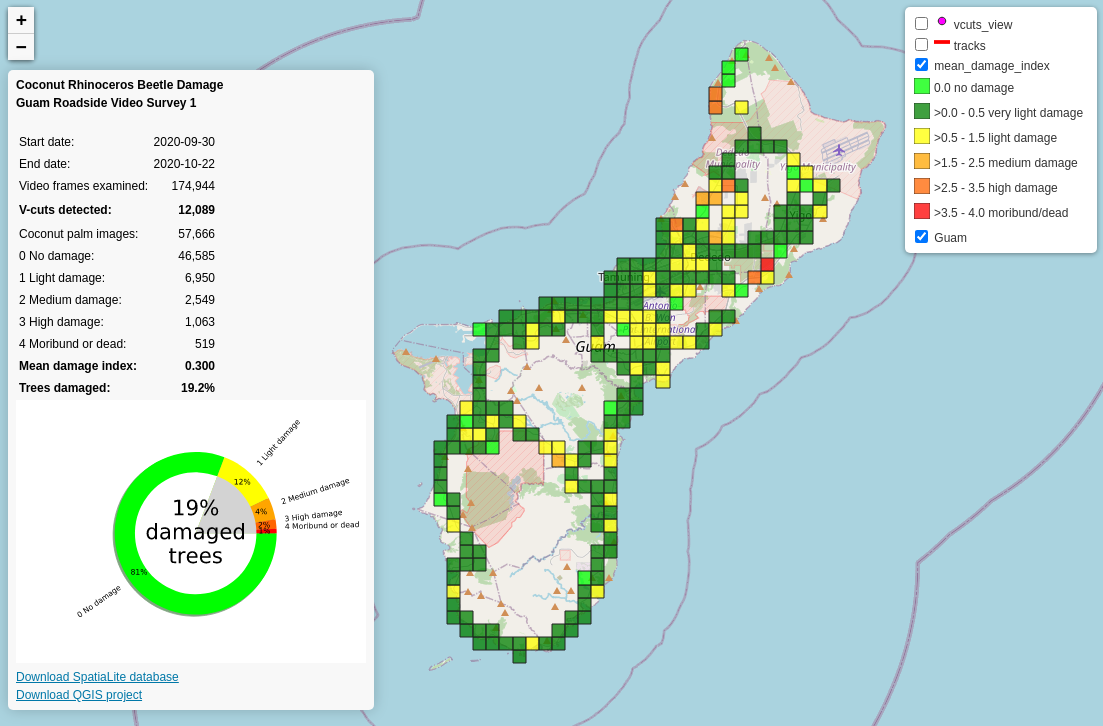
\includegraphics[width=\linewidth]{images/webmap1}
	\caption{Screenshot of an interactive web map of results from the Guam01 roadside video survey of CRB damage on Guam (\cite{mooreWebMapGuamCRBdamagemap2020102020},\cite{mooreUsingCellPhone2020}) URL: \url{https://aubreymoore.github.io/new-crb-damage-map}.}
	\label{fig:webmap1}
\end{figure}


\subsection{Methods Development}

\subsubsection{Proof of Concept}

We completed a \textit{proof of concept} trial in which deep learning algorithms were used to train an object detector which locates and counts dead and CRB-damaged coconut palms in video streams.  Visual results were presented in a YouTube post \parencite{moore_training_2019} and technical details were made available in an Open Science Framework Project \parencite{moore_open_2019}.

\subsubsection{Object Detectors for CRB Damage}

The core of our automated image analysis software for detecting CRB damage in roadside surveys a pair of object detectors, one which locates coconut palms in video frames and assigns a damage index to each palm, and another which locates v-shaped cuts to fronds in images of detected coconut palms. We use a standardized CRB damage index which is in use elsewhere in the Pacific \cite{jackson_rhinoceros_2019-1}, \cite{vaqalo_coconut_2017}.

The object detectors we used were developed by OnePanel Inc. under a contract which specified a scope of work \cite{onepanelinc.ScopeWorkObject2020} submitted in response to a request for interest (RFI) \cite{mooreRequestInterestObject2020}. The RFI contained two requirements:
\begin{enumerate}
	\item The system must be built using free open-source software (FOSS). Preferred components include Linux, OpenCV, Python, Jupyter and CVAT.
	\item The system should be designed so that it can be operated locally in early detection
	mode on remote Pacific Islands which do not have access to modern telecommunications networks.
\end{enumerate}
OnePanel incorporated the object detectors into a data processing pipeline and delivered a manual for its use cite{onepanelinc.AIPipelineOperations2020}.

\subsubsection{Survey Protocol}

Georeferenced videos were recorded using a smart phone mounted on a road vehicle. The smart phone uses a pair of free apps to record roadside videos using the phone's camera and to record location using the phone's GPS receiver. An island-wide survey is completed by driving all major routes in both directions.  For setup details see \cite{aubreymooreSetAutomatedRoadside2020}. For a nontechnical overview of the survey methods, see \cite{mooreUsingCellPhone2020}. 

\subsection{Survey Results}

\todo{add citation for slide deck}

The first island-wide roadside video survey of CRB damage on Guam was performed in early October 2020.  This survey yielded a damage index for each of 57,666 coconut palm images detected in 174,944 video frames. Nineteen percent of these palms were damaged. An online interactive map of the survey results is publicly available at \url{https://aubreymoore.github.io/new-crb-damage-map} (Fig. \ref{fig:webmap1}). All data and code used to generate the map are publicly available in a GitHub repository \url{https://github.com/aubreymoore/new-crb-damage-map}. The Guam survey will be repeated bimonthly to monitor spatial-temporal changes in CRB damage in response to control activities.

A roadside video survey of Rota Island is currently being performed to test the survey method for early detection of CRB damage in areas where this pest is not known to be established.

Moore made a presentation on the roadside survey methods and results at the December 2020 CRB-G Action Group meeting \cite{mooreVideoRecordingCRBG2020}.

\section{Regional Collaboration}

\todo{add virtual meeting info and new online resources}

An informal collaboration, the \textit{CRB-G Action Group}, has been formed among Pacific-based entomologists working on the CRB-G problem. Participants from Guam, Hawaii, Palau, Papua New Guinea, Solomon Islands, Fiji, Malaysia, Japan and New Zealand have met several times and future meetings are planned (Table \ref{tab:action-group}).  This is an \textit{ad hoc} group which has been organized by Dr. Trevor Jackson and Sean Marshall of AgResearch New Zealand. AgResearch is recognized as a global center for expertise on biological control of CRB. AgResearch scientists have worked on CRB in the south Pacific for several decades and they maintain a library of OrNV isolates in cell culture. The New Zealand government has recently committed several million dollars to aid response to CRB-G in the south Pacific islands. Although individual institutions working to find a solution to the CRB-G problem on American-affiliated islands in the northern Pacific have secured funding from multiple, short-term grants, attempts to secure funding to support a sustainable well-coordinated regional project have been unsuccessful. 

\begin{table}[h]
	\centering
	\caption{Meetings of the CRB-G Action Group}
	\begin{tabular}{l}
		\toprule
		2015 Pacific Entomology Conference, Honolulu, HI, USA \\
		2016 International Congress of Entomology, Orlando, USA \\
		2017 Japanese Society for Insect Pathology, Tokyo, Japan \\
		2018 Society for Invertebrate Pathology, Gold Coast, Australia \\
		2019 XIX International Plant Protection Congress, Hyderabad, India \\
		2020 CRB-G Action Group Annual Meeting, virtual meeting conducted as a Zoom webinar) \\
		\bottomrule
	\end{tabular}
	\label{tab:action-group}
\end{table}	

\subsection{Participation in Scientific Meetings}

Moore and Grasela participated at the XIX International Plant Protection Congress in a symposium entitled \textit{The challenge of coconut rhinoceros beetle, Oryctes rhinoceros, to palm production and prospects for control in a changing world}. Moore made an oral presentation at this meeting \parencite{moore_status_2019}.
They also participated in a CRB-G Action Group meeting with colleagues from throughout the Pacific and Asia.

Moore and Jackson organized the 2020 CRB-G Action Group meeting as a Zoom webinar which occurred on December 9, 2020. Recordings of all sections of the webinar are available online \cite{mooreVideoRecordingCRBG2020}. A presentation on automated roadside surveys of CRB damage was presented at this meeting (recording and slide deck available at \cite{mooreVideoRecordingCRBG2020} and \cite{mooreAutomatedRoadsideVideo2020}).

\subsection{Development of Online Resources}

Project resources were used to build and maintain the following:
\begin{description}
	\item[Interactive CRB Invasion History Map] \footnotesize{\url{https://aubreymoore.github.io/crbdist/mymap.html}}
	\item[CRB Wiki Site] \footnotesize{\url{https://guaminsects.net/CRBG}}
	\item[CRB-G Facebook Site] \footnotesize{\url{https://www.facebook.com/groups/crbg07}}
	\item[CRB-G ListServ (email group)] \footnotesize{\url{http://crbg.guaminsects.net/listinfo.cgi/crbg-guaminsects.net}}
	\item[CRB Action Group Reference Library] \footnotesize{\url{https://aubreymoore.pythonanywhere.com/crblib/auth/login?next=/crblib}}
\end{description}

\newpage

%\section{Appendices}
%
%\appendix
%
%\section{\label{sec:Appendix-A}Appendix A: Technical Report: Injection Bioassay
%of OrNV Isolate DUG42}
%
%See following page.
%
%%\includepdf[pages=-]{DUG42}
%
%\section{\label{sec:Appendix-B}Appendix B: Technical Report: Injection Bioassay
%of OrNV Isolate MALB}
%
%See following page.
%
%%\includepdf[pages=-]{MALB}
%
%\section{\label{sec:Appendix-C}Appendix C: Technical Report: Injection Bioassay
%of OrNV Isolate PNG}
%
%See following page.
%
%%\includepdf[pages=-]{PNG}
%
%
%\section{\label{sec:Appendix-D}Appendix D: Technical Report: Injection Bioassay
%of OrNV Isolate V23B}
%
%See following page.
%
%%\includepdf[pages=-]{V23B}
\clearpage
\printbibliography[heading=bibintoc]


\end{document}
